\chapter{Identity sites: where a cell is read}\label{ch:identity}

\section{What an identity site is}

A cell is read on sites that its healthy copies hold steadily. At such a site the healthy cell's error rate is low and the same in every
donor, so $H(\beta)$ there is the cell's healthy entropy, and a loss of fidelity moves it. These are the cell's \emph{identity sites}. They are
not markers. A marker separates one cell from others; an identity site is where one cell holds its own pattern, whether or not other cells
hold it too. The composition markers of Chapter~\ref{ch:separation} and the identity sites are disjoint by construction.

\paragraph{An image.} Picture a school in which every student has a locker. Most lockers say nothing about which year a student is
in. Some do: every student of one year keeps the same book in the same place. Those are the identity lockers. The gauge does not
count students. It walks one year's identity lockers and asks how consistently they still hold what that year's lockers hold when
all is well. A marker, by contrast, is a locker chosen because two years keep it differently. \analogy

\section{The rule}

For neutrophils on EPIC v1, from the six physical reference arrays:
\begin{enumerate}
\item the across-array standard deviation of $\beta$ is at most 0.05;
\item the mean $\beta$ lies in 0.75--0.95 (methylated channel) or 0.05--0.25 (unmethylated channel);
\item at most 3,000 sites per channel, taken in order of smallest standard deviation.
\end{enumerate}
The neutrophil set has 6,000 sites, 3,000 on each channel. \calibrated

The window keeps each site off the extremes and inside the range where entropy responds to error. $dH/d\beta=\log_2[(1-\beta)/\beta]$ is 1.58 bits per
unit $\beta$ at $\beta=0.25$ and 4.25 at $\beta=0.05$, with the same magnitudes at 0.75 and 0.95. \calc{} The same steepness is why array noise shows on
these sites (Chapter~\ref{ch:instrument}): a site near 0.95 converts a small noise in $\beta$ into a large rise in $H$.

Figure~\ref{fig:p4_window} shows where the 6,000 sites sit in the window and how their healthy spread of $H$ follows the steepness.

\begin{figure}[htbp]\centering
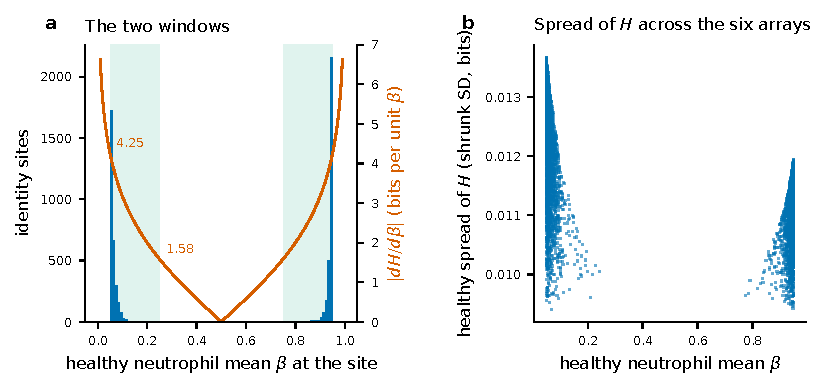
\includegraphics[width=0.95\textwidth]{figures/part6/fig_p4_15_window.pdf}
\caption{(a) Healthy neutrophil mean $\beta$ of the 6,000 identity sites, with the two windows shaded and $|dH/d\beta|$ (orange, right axis).
(b) Healthy spread of $H$ at each site across the six reference arrays (shrunk SD; median 0.0114, range 0.0094--0.0137 bits): largest
near $\beta=0.05$ and 0.95. \calibrated}
\label{fig:p4_window}
\end{figure}

\section{Why held-out readings are the only test}

The reference arrays read 1.00 by construction, because they set both the sites and the floor. That is not evidence. The evidence is an array that
played no part in choosing the sites or setting the floor, read on them, landing at 1.00 within tolerance.

\begin{center}\small
\begin{tabular}{@{}lrr@{}}\toprule
held-out reading of the six reference arrays & range & SD \\\midrule
sites re-chosen on the other five arrays & 0.983--1.045 & 0.020 \\
frozen sites, floor from the other five & 0.993--1.008 & 0.006 \\\bottomrule
\end{tabular}
\end{center}
\measured{} (SDs recomputed from the held-out record.) The difference between the two rows is selection noise: when sites are
chosen on few arrays, some enter the window by those arrays' noise, and a new array then reads off 1.00 on them. The first row is the precision the chain
prints. More physical reference arrays would shrink it.

\section{Shared sites, and what they cannot see}

Most neutrophil identity sites are held within 0.05 in $\beta$ by the other blood cells as well: 98.7~\% for monocytes, 75.6~\% for CD4 T cells
(Chapter~\ref{ch:atlas}). \calc{} Many are lineage-wide. That makes them steady across donors, and it also makes them blind to some changes. In leukaemic blood
the blasts share most of these sites, and diagnosis blood read on them stayed in Normal in 6 of 10 patients. \measured{} A blast is a progenitor, and the gauge reads a cell against its own floor; identity sites for progenitors on EPIC are not yet built. \openprob

Figure~\ref{fig:p4_shared} shows the two ends of that range.

\begin{figure}[htbp]\centering
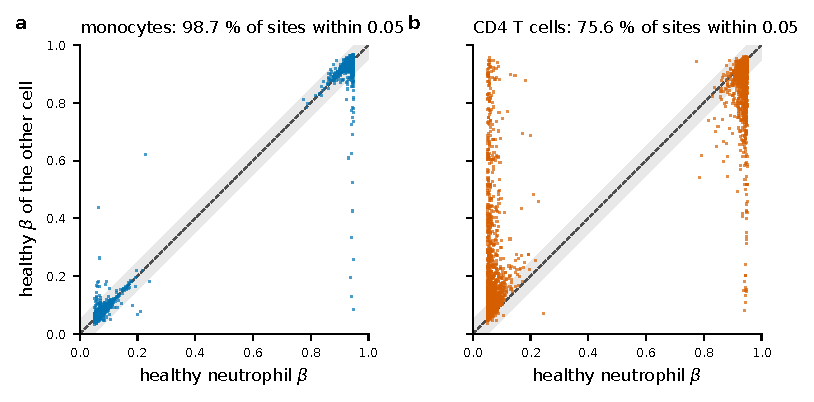
\includegraphics[width=0.85\textwidth]{figures/part6/fig_p4_15_shared.pdf}
\caption{Healthy $\beta$ of monocytes (a) and CD4 T cells (b) against neutrophils at the 6,000 identity sites; grey band: $\pm0.05$. Monocytes
hold 98.7~\% of the sites within 0.05, CD4 T cells 75.6~\%. \calc}
\label{fig:p4_shared}
\end{figure}

\paragraph{The X chromosome.} Thirty-two of the 6,000 sites lie on chrX, and they read the same on the female reference array and on the five male arrays,
because the site rule required agreement across all six (Chapter~\ref{ch:skytools}). \measured

\section{Status}

\begin{keybox}[title=Status]
One cell type has a production set of identity sites: neutrophils on EPIC v1, 6,000 sites, held-out SD 0.020. A 450K set is pending. Sets for other cell
types exist for development only and are not read by the chain. \openprob
\end{keybox}
